% Full LaTeX presentation template using beamer package, intended to be used in formal and scientific presentations
% Made in 2018 by Luis Plata: https://github.com/LuisPlata94/LaTeX-Presentation

% Based on different guides:
% ShareLaTeX's beamer guide: https://es.sharelatex.com/learn/Beamer

\documentclass[12pt]{beamer}

% Changing the appearance
\setbeamertemplate{navigation symbols}{} % Hides the navigation bar
\setbeamertemplate{caption}[numbered] % Numerates the images
\usetheme{Madrid} % Theme 
\usecolortheme{default} % Colors http://deic.uab.es/~iblanes/beamer_gallery/index_by_theme.html
%\usefonttheme{structuresmallcapsserif} % Changes font
%\usepackage{bookman} % Changes font

% Packages (General ones)
\usepackage[utf8]{inputenc} % Accents
\usepackage{blindtext} % Dummy text
\usepackage{amsthm} % Mathematical setup

% Making citations on slide:
\usepackage[style=authortitle,backend=bibtex]{biblatex}
\addbibresource{BigData.bib}

% Table of Contents
\AtBeginSection[]
{
  \begin{frame}
    \frametitle{Table of Contents}
    \tableofcontents[currentsection]
  \end{frame}
}

%Information to be included in the title page:
\title[Beamer Template] %optional
{Complete Template for a presentation in LaTeX}
 
\subtitle{Using Beamer class}
 
\author[Plata]
{Luis Fernando Plata González\inst{1}}
% Example for multiple authors {A.~B.~Arthur\inst{1} \and J.~Doe\inst{2}}
 
\institute[TEC] % (optional)
{
  \inst{1}%
  Computer Science Department\\
  Tecnológico de Monterrey
% Next lines are if multiple authors
%  \and
%  \inst{2}
%  Faculty of Chemistry\\
%  Very Famous University
}
 
\date[2018] % (optional)
{Presentation, January 2018}
 
%\logo{
\includegraphics[height=1cm]{imgs/logo_itesm.png}} % Logo on all slides
\titlegraphic{
\includegraphics[height=1.5cm]{imgs/logo_itesm.png}} % Logo on 1st slide, I use this since there are problems with the footnotes
 
\begin{document}

\frame{\titlepage}

% Table of Contents
\begin{frame}
\frametitle{Table of Contents}
\tableofcontents
\end{frame}

\section{Basic features}
\subsection{Frame with dummy text}
\begin{frame}
\frametitle{Frame example}
\blindtext[1]
\end{frame}


\subsection{Transitions}
\begin{frame}
\frametitle{Transitions with itemize}
By using itemize you add a new item per slide
 
\begin{itemize}
 \item<1-> Text visible on slide 1
 \item<2-> Text visible on slide 2
 \item<3-> Text visible on slide 3
\end{itemize}
\end{frame}

\subsection{Figures}
\begin{frame}
\frametitle{Example of a figure}
\begin{figure}[h]
	\centering
	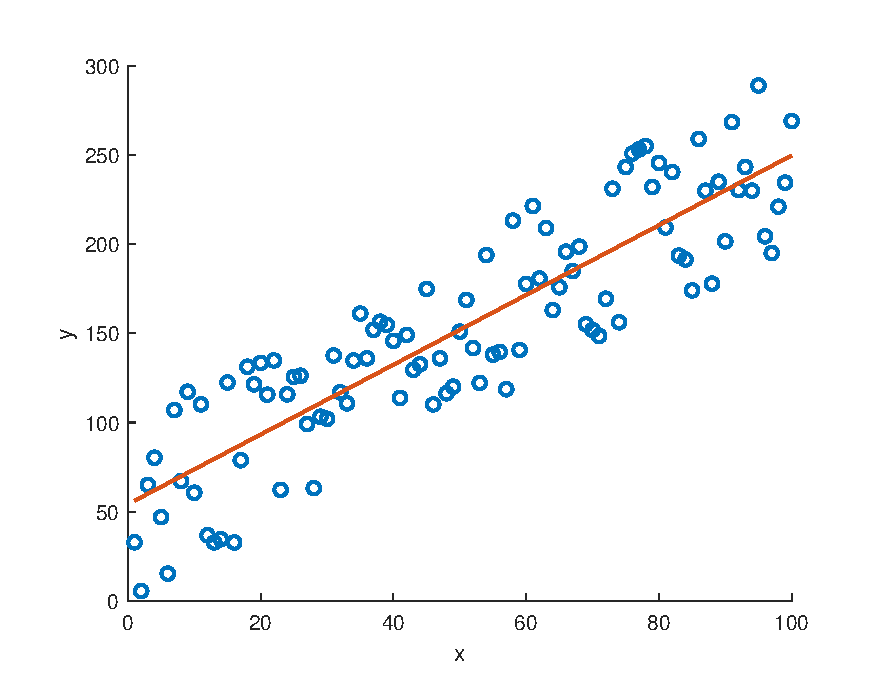
\includegraphics[width=0.6\textwidth]{imgs/r_result.eps}
	\caption{LaTeX converts .eps files to .pdf, and the resolution is conserved}
	\label{fig:1}
\end{figure}
\end{frame}

\begin{frame}
\frametitle{Transition using pause}
 In this slide \pause
 the text will be partially visible \pause
 And finally everything will be there
\end{frame}


\subsection{Highlighting text}
\begin{frame}
\frametitle{Highlighting}
 
In this slide, some important text will be
\alert{highlighted} beause it's important.
Please, don't abuse it.
 
\begin{block}{Remark}
Those colors change with the theme
\end{block}
 
\begin{alertblock}{Important theorem}
There are more types of blocks
\end{alertblock}
 
\begin{example}
Sample text in green box. "Examples" is fixed as block title.
\end{example}
\end{frame}


\subsection{Two-column slide}
\begin{frame}
\frametitle{Two-column slide}
 
\begin{columns}
 
\column{0.5\textwidth}
This is a text in first column.
$$E=mc^2$$
\begin{itemize}
\item First item
\item Second item
\end{itemize}
 
\column{0.5\textwidth}
This text will be in the second column
and on a second tought this is a nice looking
layout in some cases.
\end{columns}
\end{frame}


\end{document}

